% =====================================================================
%  Apresentação da defesa do TCC — modelo IFC Videira (Beamer)
%  Compilar:  latexmk -pdf main.tex     (pdfLaTeX + Biber)
%  Usa ../referencias.bib, ../figuras/ e ../images/ do texto do TCC.
%  Roteiro de fala: roteiro.md
% =====================================================================
\documentclass[aspectratio=169,11pt,xcolor=table]{beamer}
\usepackage[T1]{fontenc}
\usepackage[utf8]{inputenc}
\usepackage[brazil]{babel}
\usepackage{csquotes}
\usepackage[style=abnt,backend=biber]{biblatex}
\addbibresource{../referencias.bib}
% o .bib do TCC escapa "_" nas URLs (\_), o que o biblatex imprime como %5C_
\DeclareSourcemap{\maps[datatype=bibtex]{\map{\step[fieldsource=url, match=\regexp{\\\_}, replace=\regexp{\_}]}}}
% ponytail: nos slides, DOI basta; URL só quando não houver DOI
\AtEveryBibitem{\iffieldundef{doi}{}{\clearfield{url}\clearfield{urlyear}\clearfield{urlmonth}\clearfield{urlday}}}
\renewcommand*{\bibfont}{\scriptsize}
\setlength\bibitemsep{0.3em}
\usepackage{pgfplots}
\pgfplotsset{compat=1.18, /pgf/number format/use comma, /pgf/number format/1000 sep={.}}
\usetikzlibrary{positioning,arrows.meta,fit,backgrounds,calc}

\usetheme{IFCVideira}
\graphicspath{{figuras/}{../images/}}

% Estilos usados pelas figuras TikZ do TCC (../figuras), nas cores do tema
\tikzset{
  caixa/.style={draw=ifcescuro, rounded corners=2pt, align=center, font=\footnotesize,
                minimum height=0.9cm, inner sep=4pt, fill=white},
  ia/.style={caixa, draw=ifcverde, fill=ifcclaro, line width=0.8pt},
  ext/.style={caixa, dashed},
  seta/.style={-{Stealth[length=2.2mm]}, thick, draw=ifcescuro},
  grupo/.style={draw, rounded corners=4pt, inner sep=8pt, dashed, ifccinza},
  rotulo/.style={font=\scriptsize\itshape, align=center, text=ifccinza}
}
\newcommand{\st}[1]{{\bfseries\color{#1}}}
\newcommand{\ok}{{\bfseries\color{ifcverde}OK}}
\newcommand{\inc}{{\bfseries\color{ifcamarelo}INCOMPLETO}}
\newcommand{\aus}{{\bfseries\color{ifcvermelho}AUSENTE}}
\newcommand{\numero}[2]{{\fontsize{26}{30}\selectfont\bfseries\color{ifcverde}#1\par}\smallskip{\small\color{ifccinza}#2\par}}

% ---------------- Dados do trabalho ----------------
\title{Sistema de suporte à validação de planos de ensino com modelos de linguagem}
\author{Vinícius Slongo}
\orientador{Prof. Me. Fabricio Bizotto}
\local{Videira (SC)}
\date{novembro de 2026}
% ---------------------------------------------------

\begin{document}

\capa

\begin{frame}{Roteiro da apresentação}
  \begin{columns}[T]
    \begin{column}{0.45\textwidth}
      \begin{enumerate}\setlength\itemsep{1.2em}
        \item Introdução
        \item Fundamentação teórica
        \item Metodologia
      \end{enumerate}
    \end{column}
    \begin{column}{0.45\textwidth}
      \begin{enumerate}\setcounter{enumi}{3}\setlength\itemsep{1.2em}
        \item Desenvolvimento
        \item Resultados e discussão
        \item Considerações finais
      \end{enumerate}
    \end{column}
  \end{columns}
\end{frame}

% =====================================================================
\secao[Contexto, problema de pesquisa e objetivos]{Introdução}
% =====================================================================

\begin{frame}{Contextualização e problema}
  \begin{columns}[T]
    \begin{column}{0.54\textwidth}
      \begin{itemize}\small\setlength\itemsep{0.45em}
        \item A Organização Didática define o que o plano de ensino deve conter \cite{ifc2022}
        \item Conferência \textbf{manual}: coordenação e NDE leem plano por plano
        \item Repetitiva e sujeita a \textbf{inconsistências entre avaliadores}
        \item SIGAA padroniza as seções, mas o conteúdo é texto livre
        \item LLMs interpretam texto, mas \textbf{alucinam} \cite{Ji2023}
      \end{itemize}
    \end{column}
    \begin{column}{0.4\textwidth}
      \begin{cartao}[title={Regras fixas resolvem\ldots}]
        \small ``A seção existe?'' \quad ``Há 3 referências básicas?''
      \end{cartao}
      \medskip
      \begin{cartao}[title={\ldots mas não julgam}]
        \small ``Esta metodologia descreve \emph{como} as aulas serão conduzidas?''
      \end{cartao}
    \end{column}
  \end{columns}
\end{frame}

\begin{frame}{Problema de pesquisa e objetivos}
  \vspace{-0.2cm}
  \begin{cartao}[title={Problema de pesquisa}]
    \footnotesize De que forma um sistema baseado em modelos de linguagem pode apoiar a verificação
    da conformidade dos planos de ensino às normas do IFC, indicando de forma confiável os
    itens que exigem revisão e preservando o controle humano sobre a decisão final?
  \end{cartao}
  \smallskip
  \begin{columns}[T]
    \begin{column}{0.38\textwidth}
      {\usebeamercolor[fg]{example text}\bfseries Objetivo geral}\par\smallskip
      \footnotesize Desenvolver e avaliar um sistema semiautomático baseado em IA para apoiar a
      validação dos planos de ensino do curso de Ciência da Computação do IFC Videira.
    \end{column}
    \begin{column}{0.58\textwidth}
      {\usebeamercolor[fg]{example text}\bfseries Objetivos específicos}\par\smallskip
      \begin{enumerate}\footnotesize\setlength\itemsep{0.15em}
        \item Converter a Organização Didática em critérios verificáveis
        \item Implementar um \textit{pipeline} com LLM local e registro rastreável
        \item Disponibilizar um painel \textit{web} com resultado e justificativa
        \item Avaliar com planos reais (2024/1 a 2025/2): robustez, desempenho e concordância
      \end{enumerate}
    \end{column}
  \end{columns}
\end{frame}

% =====================================================================
\secao[Conceitos que sustentam o trabalho]{Fundamentação teórica}
% =====================================================================

\begin{frame}{Como tornar as respostas de um LLM confiáveis}
  \begin{columns}[T]
    \begin{column}{0.48\textwidth}
      \begin{itemize}\setlength\itemsep{0.6em}
        \item \textbf{Saída estruturada}: um esquema JSON restringe a decodificação e
              garante a estrutura da resposta \cite{Willard2023}
        \item \textbf{Regras determinísticas}: o que é exato (contar, detectar campo vazio)
              fica com o código
        \item \textbf{LLM como avaliador}: boa concordância com humanos, mas com vieses
              \cite{Zheng2023}
      \end{itemize}
    \end{column}
    \begin{column}{0.48\textwidth}
      \begin{itemize}\setlength\itemsep{0.6em}
        \item \textbf{Execução local} (Ollama + Qwen2.5 7B quantizado): sem custo por
              requisição e sem enviar documentos para fora --- LGPD \cite{Brasil2018}
        \item \textbf{IA centrada no humano}: o sistema aponta, o avaliador decide
              \cite{Shneiderman2022}
      \end{itemize}
    \end{column}
  \end{columns}
\end{frame}

\begin{frame}{Trabalhos relacionados}
  \begin{table}
    \caption{Comparativo entre trabalhos relacionados}
    \tiny
    \renewcommand{\arraystretch}{1.2}
    \begin{tabular}{L{3.6cm}L{4.0cm}L{2.9cm}L{3.4cm}}
      \rowcolor{ifcescuro}
      \textcolor{white}{\textbf{Trabalho}} & \textcolor{white}{\textbf{Foco}} &
      \textcolor{white}{\textbf{Tipo de estudo}} & \textcolor{white}{\textbf{Processo administrativo?}} \\
      \textcite{Tan2025}       & IA no ensino e formação docente & Revisão sistemática & Apontado como lacuna \\ \hline
      \textcite{Kasneci2023}   & Oportunidades e riscos de LLMs  & Ensaio crítico      & Não \\ \hline
      \textcite{Sposato2025}   & IA na gestão educacional        & Taxonomia           & Sim, conceitual \\ \hline
      \textcite{Hoare2025}     & Ferramenta institucional de IA  & Relato de implantação & Não \\ \hline
      \textcite{Santos2025}    & Plataformas e IA na gestão pública & Análise documental & Sim, conceitual \\ \hline
      \textcite{Vieira2025}    & IA nos Institutos Federais      & Revisão integrativa & Apontado como lacuna \\ \hline
      \rowcolor{ifcclaro}
      \textcolor{ifcverdeesc}{\textbf{Este trabalho}} & \textcolor{ifcverdeesc}{\textbf{Validação de planos de ensino}} &
      \textcolor{ifcverdeesc}{\textbf{Sistema e estudo de caso}} & \textcolor{ifcverdeesc}{\textbf{Sim, implementado e avaliado}} \\
    \end{tabular}
    \fonte{Elaborado pelo autor (2026).}
  \end{table}
\end{frame}

% =====================================================================
\secao[Como o trabalho foi desenvolvido e avaliado]{Metodologia}
% =====================================================================

\begin{frame}{Classificação, corpus e ambiente}
  \begin{columns}[T]
    \begin{column}{0.48\textwidth}
      \begin{itemize}\setlength\itemsep{0.55em}
        \item Pesquisa \textbf{aplicada}, exploratória e descritiva \cite{Gil2017}
        \item \textbf{Estudo de caso} \cite{Yin2015}; unidade de análise:
              (plano, critério)
        \item Desenvolvimento \textbf{iterativo e incremental} (maio a novembro/2026)
        \item \textbf{Corpus}: 29 planos de 2024/1 (avaliação detalhada) e 120 de 2024/1 a 2025/2 (ampliação)
        \item Resultados anonimizados (P01 a P29)
      \end{itemize}
    \end{column}
    \begin{column}{0.46\textwidth}
      \begin{cartao}[title={Ambiente experimental}]
        \footnotesize
        \begin{tabular}{@{}ll@{}}
          CPU & Intel Core Ultra 7 155H \\
          GPU & RTX 4050 Laptop, 6 GB \\
          RAM & 32 GB \\
          Orquestração & n8n 2.21 (Docker) \\
          Inferência & Ollama 0.24 \\
          Modelo & Qwen2.5 7B, Q4\_K\_M \\
          Temperatura & 0,1 \\
        \end{tabular}
      \end{cartao}
    \end{column}
  \end{columns}
\end{frame}

\begin{frame}{Doze critérios de avaliação}
  \centering\scriptsize
  \renewcommand{\arraystretch}{1.05}
      \begin{tabular}{L{4.2cm}L{7.2cm}L{1.2cm}}
        \rowcolor{ifcescuro}
        \textcolor{white}{\textbf{Critério}} & \textcolor{white}{\textbf{Regra para OK}} & \textcolor{white}{\textbf{Por}} \\
        Identificação          & Instituição, componente e docente & LLM \\
        Ementa                 & Texto corrido, $\geq$ 15 palavras & LLM \\
        Objetivo geral / específicos & Texto preenchido            & Regra \\
        Conteúdo programático  & Lista tópicos ou unidades         & LLM \\
        Metodologia            & Estratégias e recursos das aulas  & LLM \\
        Proc. de avaliação / Avaliações & Instrumentos, datas ou pesos & LLM \\
        Cronograma             & Distribuição por datas ou semanas & LLM \\
        Horário de atendimento & Dia(s) e/ou horário(s)            & LLM \\
        \rowcolor{ifcclaro}
        Referências            & $\geq$ 3 básicas e $\geq$ 5 complementares & Regra \\
        Coerência              & Objetivos, metodologia e avaliação compatíveis & LLM \\
      \end{tabular}
  \fonte{Elaborado pelo autor (2026), com base em \textcite{ifc2022}.}
  \medskip
  \raggedright\scriptsize
  {\usebeamercolor[fg]{example text}\bfseries Critério:}\enspace
  \ok{} atende \quad \inc{} há conteúdo, mas não atende \quad \aus{} vazio ou sem relação\par\smallskip
  {\usebeamercolor[fg]{example text}\bfseries Plano:}\enspace
  \ok{} tudo OK \quad {\bfseries\color{ifcamarelo}PENDENTE} algum INCOMPLETO \quad
  {\bfseries\color{ifcvermelho}REPROVADO} algum AUSENTE \quad {\bfseries\color{ifccinza}ERRO} falha técnica
\end{frame}

\begin{frame}{Protocolo de avaliação}
  \vspace{0.3cm}
  \begin{tikzpicture}[x=1cm,y=1cm,
      etapa/.style={fill=ifcclaro,rounded corners=2mm,minimum width=3.4cm,minimum height=3.9cm},
      num/.style={circle,fill=ifcverde,text=white,font=\bfseries,minimum size=0.85cm,inner sep=0}]
    \foreach \i/\t/\d in {
        0/Robustez/{Proporção de planos com status ERRO em cada iteração},
        1/Desempenho/{Tempo de inferência por plano e do lote, \textit{tokens}/s (metadados do Ollama)},
        2/Concordância/{Horário de atendimento \textit{vs.} oráculo estrutural: precisão, \textit{recall}, Kappa},
        3/Análise de erros/{Todo apontamento diferente de OK conferido no texto do PDF}} {
      \pgfmathsetmacro{\x}{\i*3.62}
      \node[etapa,anchor=north west] at (\x,0) {};
      \node[num,anchor=north west] at (\x+0.3,-0.3) {\pgfmathparse{int(\i+1)}\pgfmathresult};
      \node[anchor=north west,font=\bfseries,text=ifcescuro] at (\x+0.22,-1.35) {\t};
      \node[anchor=north west,text width=2.95cm,align=left,font=\scriptsize] at (\x+0.22,-1.9) {\d};
    }
  \end{tikzpicture}
\end{frame}

% =====================================================================
\secao[Arquitetura, fluxo de validação e interface]{Desenvolvimento}
% =====================================================================

\begin{frame}{Arquitetura do sistema}
  % ponytail: versão simplificada de ../figuras/arquitetura, legível no projetor
  \begin{figure}
    \caption{Arquitetura do sistema}
    \begin{tikzpicture}[every node/.style={font=\footnotesize}, node distance=0.9cm and 1.1cm]
      \node[ext, text width=2.3cm] (planos) {Pasta \texttt{planos}\\\scriptsize PDFs};
      \node[caixa, text width=3.2cm, right=of planos] (val) {\textbf{Workflow de validação}\\\scriptsize extrai, segmenta, monta \textit{prompt}, aplica regras};
      \node[ia, text width=2.8cm, right=2.1cm of val] (llm) {\textbf{Ollama}\\\scriptsize Qwen2.5 7B na GPU (6 GB)};
      \node[ext, text width=2.3cm, below=of planos] (res) {Pasta \texttt{resultados}\\\scriptsize um JSON por plano};
      \node[caixa, text width=3.2cm, right=of res] (dash) {\textbf{Workflow do \textit{dashboard}}\\\scriptsize HTML e CSV};
      \node[caixa, text width=2.8cm, right=2.1cm of dash] (user) {Coordenação / NDE\\\scriptsize navegador \textit{web}};
      \draw[seta] (planos) -- (val);
      \draw[seta] ([yshift=2mm]val.east) -- node[rotulo, above]{\textit{prompt} + esquema} ([yshift=2mm]llm.west);
      \draw[seta] ([yshift=-2mm]llm.west) -- node[rotulo, below]{JSON} ([yshift=-2mm]val.east);
      \draw[seta] (val.south west) -- (res.north east);
      \draw[seta] (res) -- (dash);
      \draw[seta, {Stealth[length=2.2mm]}-{Stealth[length=2.2mm]}] (dash) -- (user);
      \begin{scope}[on background layer]
        \node[grupo, fit=(val)(dash), inner sep=6pt, label={[font=\scriptsize\bfseries,text=ifccinza]above:Contêiner n8n}] {};
        \node[grupo, fit=(llm), inner sep=6pt, label={[font=\scriptsize\bfseries,text=ifccinza]above:Contêiner Ollama}] {};
      \end{scope}
    \end{tikzpicture}
    \fonte{Elaborado pelo autor (2026).}
  \end{figure}
\end{frame}

\begin{frame}{Fluxo de validação no n8n}
  \begin{figure}
    \caption{Etapas do fluxo de validação}
    \resizebox{!}{4.7cm}{\begin{tikzpicture}[node distance=0.55cm, every node/.style={font=\scriptsize}]
  \tikzset{no/.style={caixa, font=\scriptsize, minimum width=2.25cm, minimum height=1.1cm, text width=2.05cm}}
  % Linha 1: aquisição
  \node[no] (n1) {\textbf{Gatilho}\\agendado (5h) ou manual};
  \node[no, right=of n1] (n2) {\textbf{Buscar arquivos}\\pasta do Drive};
  \node[no, right=of n2] (n3) {\textbf{Baixar arquivo}\\binário do PDF};
  \node[no, right=of n3] (n4) {\textbf{Filtrar tipo}\\somente PDF};
  \node[no, right=of n4] (n5) {\textbf{Extrair texto}\\PDF.js};
  % Linha 2: processamento
  \node[no, below=1.5cm of n5] (n6) {\textbf{Separar por tópicos}\\regex + contagem de referências};
  \node[no, left=of n6] (n7) {\textbf{Preparar \textit{prompt}}\\regras + esquema JSON};
  \node[no, left=of n7] (n8) {\textbf{Processar em blocos}\\10 planos por vez};
  \node[ia, no, left=of n8] (n9) {\textbf{Validar com IA}\\Ollama, 1 req./vez};
  \node[no, left=of n9] (n10) {\textbf{Interpretar}\\regras determinísticas};
  \node[no, below=1.2cm of n10] (n11) {\textbf{Registrar}\\Google Sheets};

  \foreach \a/\b in {n1/n2,n2/n3,n3/n4,n4/n5,n6/n7,n7/n8,n9/n10,n10/n11} \draw[seta] (\a) -- (\b);
  \draw[seta] (n5) -- (n6);
  \draw[seta] (n8) -- (n9);
  \draw[seta] (n11.east) -| node[rotulo, pos=0.25, below]{próximo bloco} (n8.south);

  \node[grupo, fit=(n1)(n5), label={[font=\footnotesize\bfseries]above:Aquisição}] {};
  \node[grupo, fit=(n6)(n10)(n11), label={[font=\footnotesize\bfseries]below:Análise e registro}] {};
\end{tikzpicture}
}
    \fonte{Elaborado pelo autor (2026).}
  \end{figure}
\end{frame}

\begin{frame}{Painel de resultados (\textit{dashboard})}
  \begin{columns}[T]
    \begin{column}{0.4\textwidth}
      \begin{itemize}\small\setlength\itemsep{0.6em}
        \item Indicadores do lote: aprovados, pendentes, com problemas
        \item Um cartão por plano, com os 12 critérios e a justificativa de cada um
        \item Cor \textbf{e} texto do status (acessibilidade)
        \item Atalho para o PDF original e exportação em CSV
        \item Exemplo: P05 --- faltam horário e objetivos específicos
      \end{itemize}
    \end{column}
    \begin{column}{0.56\textwidth}
      \centering
      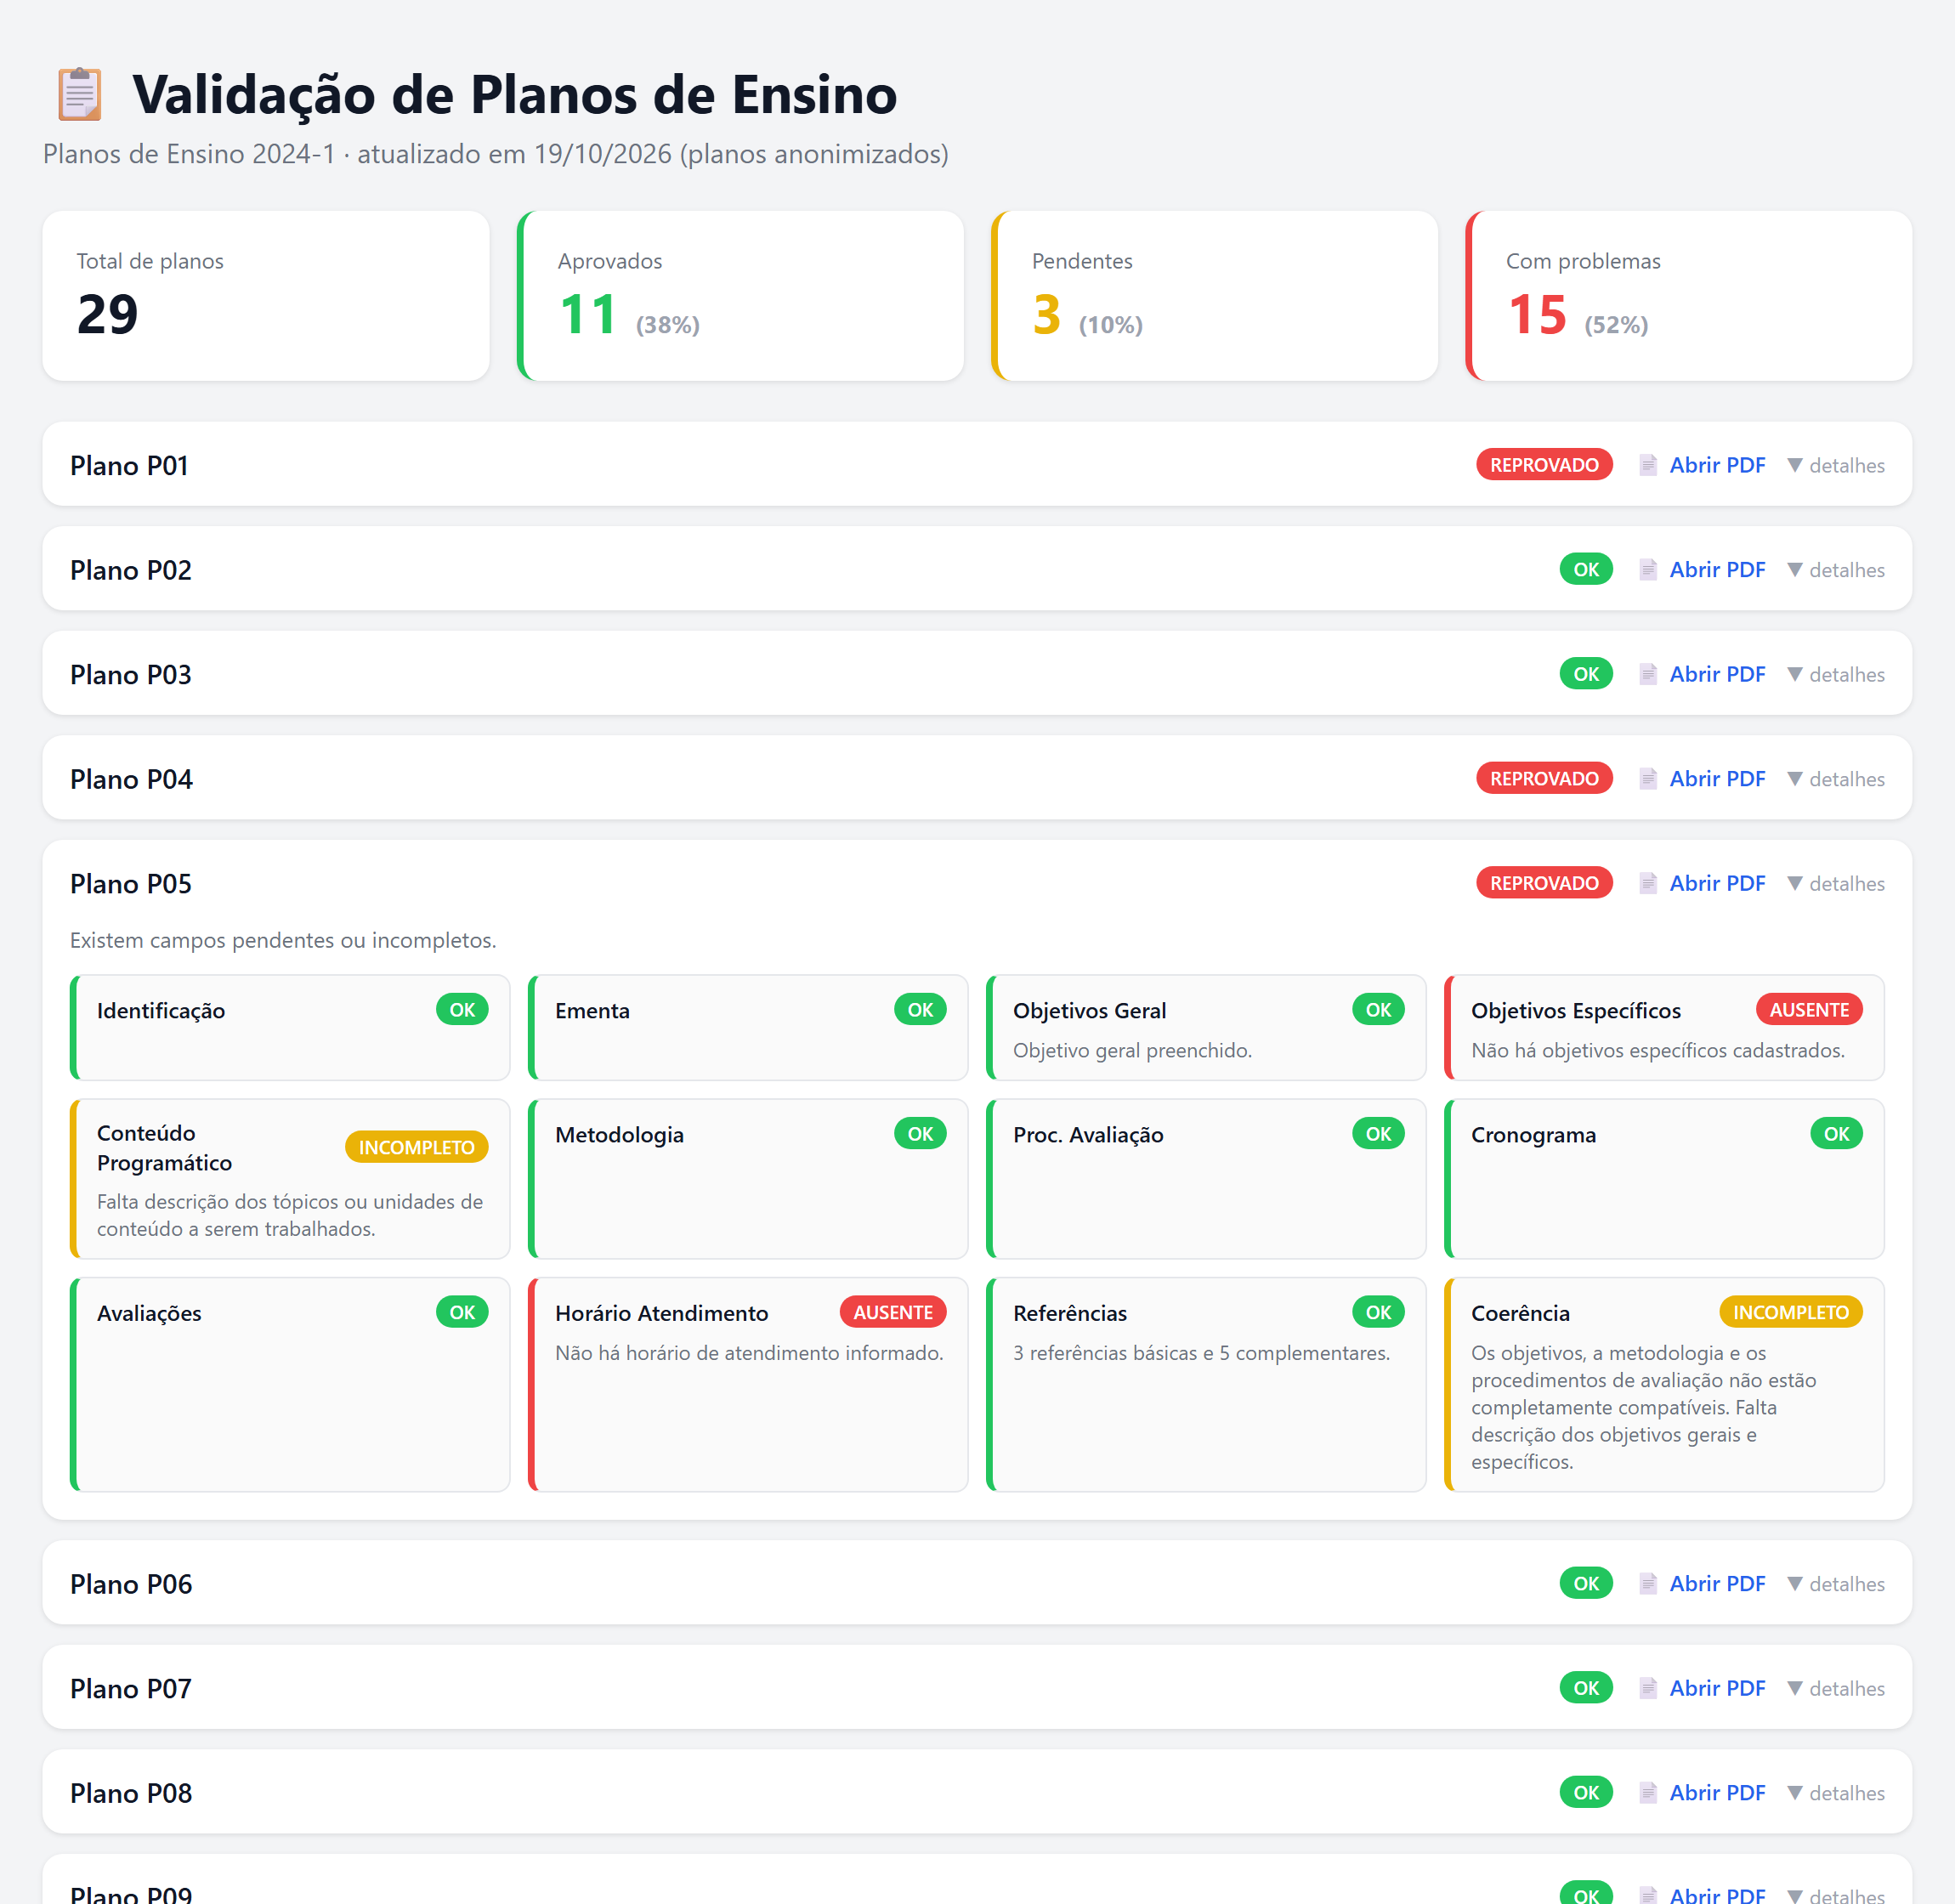
\includegraphics[height=5.8cm]{dashboard}
      \fonte{Elaborado pelo autor (2026). Nomes anonimizados.}
    \end{column}
  \end{columns}
\end{frame}

% =====================================================================
\secao[O que foi obtido e o que isso significa]{Resultados e discussão}
% =====================================================================

\begin{frame}{Robustez técnica ao longo das iterações}
  \begin{columns}[T]
    \begin{column}{0.56\textwidth}
      \begin{figure}
        \caption{Planos com status ERRO por execução (\%)}
        \begin{tikzpicture}
          \begin{axis}[ybar, width=\linewidth, height=5.4cm, ymin=0, ymax=100,
              bar width=0.55cm, axis y line=none, axis x line*=bottom, bar shift=0pt,
              symbolic x coords={22/05,07/07,10/08,25/08,10/09,15/09,19/10},
              xtick={22/05,07/07,10/08,25/08,10/09,15/09,19/10},
              nodes near coords={\pgfmathprintnumber[fixed,precision=1]{\pgfplotspointmeta}},
              every node near coord/.append style={font=\tiny},
              x tick label style={font=\tiny}, enlarge x limits=0.08]
            \addplot[fill=ifccinza,draw=none] coordinates
              {(22/05,86.2) (07/07,3.4) (10/08,69.0) (25/08,49.1) (10/09,0) (15/09,17.2)};
            \addplot[fill=ifcverde,draw=none] coordinates {(19/10,0)};
          \end{axis}
        \end{tikzpicture}
        \fonte{Elaborado pelo autor (2026).}
      \end{figure}
    \end{column}
    \begin{column}{0.4\textwidth}
      \scriptsize
      \renewcommand{\arraystretch}{1.25}
      \begin{tabular}{L{2.2cm}L{3.3cm}}
        \rowcolor{ifcescuro}
        \textcolor{white}{\textbf{Falha}} & \textcolor{white}{\textbf{Correção}} \\
        JSON vazio/truncado & Uma requisição por vez + 3 tentativas \\ \hline
        JSON malformado & Saída estruturada (esquema) \\ \hline
        \textit{Prompt} cortado em silêncio (4.096 \textit{tokens}) & Contexto explícito + \textit{prompt} menor \\ \hline
        \textit{Timeout} & \textit{FlashAttention}, \textit{KV cache} 8 bits \\
      \end{tabular}
      \par\medskip
      \numero{86,2\% \(\rightarrow\) 0\%}{de planos com falha técnica}
    \end{column}
  \end{columns}
\end{frame}

\begin{frame}{Desempenho: 120 planos, 4x mais lento com a GPU disputada}
  \begin{columns}[T]
    \begin{column}{0.3\textwidth}
      \numero{46 s}{por plano na execução dos 120 planos (mediana 41 s; 28 a 77 s)}
    \end{column}
    \begin{column}{0.3\textwidth}
      \numero{11,5 s}{por plano em 19/10, com a GPU livre (29 planos em 8 min 54 s)}
    \end{column}
    \begin{column}{0.3\textwidth}
      \numero{14\%}{do modelo na CPU em 04/11 (8\% em 19/10): outros programas usavam a GPU}
    \end{column}
  \end{columns}
  \vspace{0.8cm}
  \begin{itemize}\small\setlength\itemsep{0.5em}
    \item A lentidão expôs uma falha: o fluxo envia um plano por segundo sem esperar a resposta;
          55 planos estouraram o tempo limite e foram reprocessados
    \item Com a GPU livre, centenas de planos caberiam em menos de 1 hora, de madrugada
    \item Sem custo por requisição e sem enviar documentos para fora
  \end{itemize}
\end{frame}

\begin{frame}{Horário de atendimento falhou em 69 dos 120 planos}
  \begin{columns}[T]
    \begin{column}{0.6\textwidth}
      \begin{figure}
        \caption{Resultado por critério, 2024/1 a 2025/2 (n.º de planos)}
        \begin{tikzpicture}
          \begin{axis}[xbar stacked, width=0.82\linewidth, height=5.3cm, bar width=5pt,
              xmin=0, xmax=120, axis x line*=bottom,
              xtick={0,30,60,90,120}, ytick=data, y dir=reverse,
              yticklabels={Identificação,Ementa,Objetivo geral,Obj. específicos,Conteúdo,Metodologia,Proc. avaliação,Cronograma,Avaliações,Horário de atendimento,Referências,Coerência},
              y tick label style={font=\tiny}, x tick label style={font=\tiny},
              axis y line*=left, y axis line style={draw=none}, ytick style={draw=none},
              legend style={at={(0.5,-0.1)},anchor=north,legend columns=3,font=\tiny,draw=none},
              enlarge y limits=0.05]
            \addplot[fill=ifcverde,draw=none] coordinates {(120,1) (114,2) (120,3) (104,4) (118,5) (119,6) (116,7) (119,8) (113,9) (51,10) (103,11) (117,12)};
            \addplot[fill=ifcamarelo,draw=none] coordinates {(0,1) (6,2) (0,3) (15,4) (0,5) (1,6) (4,7) (1,8) (6,9) (7,10) (17,11) (3,12)};
            \addplot[fill=ifcvermelho,draw=none] coordinates {(0,1) (0,2) (0,3) (1,4) (2,5) (0,6) (0,7) (0,8) (1,9) (62,10) (0,11) (0,12)};
            \legend{OK, INCOMPLETO, AUSENTE}
          \end{axis}
        \end{tikzpicture}
        \fonte{Elaborado pelo autor (2026).}
      \end{figure}
    \end{column}
    \begin{column}{0.36\textwidth}
      \footnotesize
      {\bfseries\color{ifcverde}36 OK (30\%)}\\
      {\bfseries\color{ifcamarelo}21 pendentes (17,5\%)}\\
      {\bfseries\color{ifcvermelho}63 reprovados (52,5\%)}
      \par\medskip
      \begin{itemize}\setlength\itemsep{0.45em}
        \item \textbf{Horário de atendimento} não conforme em 69 planos: em 43, é o único problema
        \item Referências incompletas em 17; objetivos específicos em 16
        \item Problema \textbf{sistemático} do curso, repetido nos quatro semestres
      \end{itemize}
    \end{column}
  \end{columns}
\end{frame}

\begin{frame}{Em 2024/1, contra o oráculo estrutural, o Kappa foi de 0,93}
  \begin{columns}[T]
    \begin{column}{0.52\textwidth}
      \small Oráculo: no PDF do SIGAA, o texto entre ``Horário de Atendimento'' e
      ``Programa'' indica se o campo foi preenchido.
      \par\medskip
      \scriptsize
      \renewcommand{\arraystretch}{1.4}
      \begin{tabular}{lcc}
        \rowcolor{ifcescuro}
        & \textcolor{white}{\textbf{Sist.: não conf.}} & \textcolor{white}{\textbf{Sist.: conforme}} \\
        \textbf{Oráculo: vazio}      & \cellcolor{ifcclaro}15 (VP) & 0 (FN) \\
        \textbf{Oráculo: preenchido} & 1 (FP) & \cellcolor{ifcclaro}13 (VN) \\
      \end{tabular}
      \fonte{Elaborado pelo autor (2026).}
    \end{column}
    \begin{column}{0.2\textwidth}
      \numero{100\%}{\textit{recall}}\bigskip
      \numero{93,8\%}{precisão}
    \end{column}
    \begin{column}{0.22\textwidth}
      \numero{0,93}{Kappa de Cohen: quase perfeita \cite{Landis1977}}\bigskip
      \numero{0,968}{$F_1$}
    \end{column}
  \end{columns}
  \vspace{0.3cm}
  {\small O único FP (P19, ``conforme horário disponibilizado publicamente'') é de fato não conforme pela regra.}
\end{frame}

\begin{frame}{Análise de erros}
  \begin{columns}[T]
    \begin{column}{0.48\textwidth}
      {\usebeamercolor[fg]{example text}\bfseries O que funcionou}\par\medskip
      \begin{itemize}\small\setlength\itemsep{0.5em}
        \item Os 11 demais apontamentos verificados no PDF eram \textbf{não conformidades reais}
        \item O modelo detecta bem \emph{se} há problema
      \end{itemize}
    \end{column}
    \begin{column}{0.48\textwidth}
      {\color{ifcvermelho}\bfseries O que falhou}\par\medskip
      \begin{itemize}\small\setlength\itemsep{0.5em}
        \item Instável entre \inc{} e \aus{}: P20 e P21, quase idênticos, terminaram
              REPROVADO e PENDENTE
        \item \textbf{1 falso negativo} da \emph{regra}, não do modelo: ``Não Cadastrado!''
              aceito como objetivo geral (P05)
        \item Observação geral contradiz o critério de referências em 18 de 24 planos
      \end{itemize}
    \end{column}
  \end{columns}
\end{frame}

\begin{frame}{Por semestre: desde 2024/2, o link do PTD substitui o horário}
  \begin{columns}[T]
    \begin{column}{0.5\textwidth}
      \begin{figure}
        \caption{Status geral por semestre (n.º de planos)}
        \begin{tikzpicture}
          \begin{axis}[ybar stacked, width=\linewidth, height=5.2cm, bar width=0.65cm,
              ymin=0, ymax=36, axis y line=none, axis x line*=bottom,
              symbolic x coords={2024/1,2024/2,2025/1,2025/2}, xtick=data,
              nodes near coords, every node near coord/.append style={font=\tiny},
              x tick label style={font=\scriptsize}, enlarge x limits=0.2,
              legend style={at={(0.5,-0.15)},anchor=north,legend columns=3,font=\tiny,draw=none}]
            \addplot[fill=ifcverde,draw=none] coordinates {(2024/1,11) (2024/2,12) (2025/1,5) (2025/2,8)};
            \addplot[fill=ifcamarelo,draw=none] coordinates {(2024/1,4) (2024/2,8) (2025/1,5) (2025/2,4)};
            \addplot[fill=ifcvermelho,draw=none,every node near coord/.append style={text=white}] coordinates {(2024/1,14) (2024/2,14) (2025/1,19) (2025/2,16)};
            \legend{OK, PENDENTE, REPROVADO}
          \end{axis}
        \end{tikzpicture}
        \fonte{Elaborado pelo autor (2026).}
      \end{figure}
    \end{column}
    \begin{column}{0.46\textwidth}
      \begin{itemize}\small\setlength\itemsep{0.45em}
        \item Reprovados por semestre: 48\%, 41\%, 66\% e 57\%
        \item 29 planos trazem só o \textbf{link da página de PTD}, sem dia nem hora
        \item Pela regra, o sistema acertou os 120; errou a categoria (AUSENTE em vez de INCOMPLETO)
        \item Aceitar o link é decisão do NDE: reprovados cairiam de \textbf{63 para 30}
        \item 2024/1 reprocessado: \textbf{99,2\%} das classificações iguais
      \end{itemize}
    \end{column}
  \end{columns}
\end{frame}

% =====================================================================
\secao[Conclusões e próximos passos]{Considerações finais}
% =====================================================================

\begin{frame}{Considerações finais}
  \begin{columns}[T]
    \begin{column}{0.5\textwidth}
      {\usebeamercolor[fg]{example text}\bfseries\large Conclusões}\par\medskip
      \begin{itemize}\small\setlength\itemsep{0.5em}
        \item Os quatro objetivos específicos foram atendidos
        \item Sistema \textbf{viável como triagem}: aponta planos e itens a revisar;
              a decisão fica com o avaliador
        \item A confiabilidade veio mais da \textbf{engenharia em torno do modelo}
              do que do modelo em si
        \item Regras para o exato, LLM para o interpretativo --- e as regras também
              precisam ser validadas
      \end{itemize}
    \end{column}
    \begin{column}{0.44\textwidth}
      {\usebeamercolor[fg]{example text}\bfseries\large Limitações}\par\medskip
      \begin{itemize}\small\setlength\itemsep{0.5em}
        \item Sem anotação humana completa (NDE): oráculo em um único critério
        \item Avaliação detalhada em um semestre; ampliação em um único curso
        \item Planos digitalizados (sem texto) não são lidos
        \item Dependência do formato do SIGAA
        \item Tempo economizado não foi medido
      \end{itemize}
    \end{column}
  \end{columns}
\end{frame}

\begin{frame}{Trabalhos futuros}
  \begin{enumerate}\setlength\itemsep{0.8em}
    \item Executar o protocolo de anotação com o NDE em todos os critérios e ampliar o corpus
    \item Atribuir \aus{} por regra a campos vazios e provisórios (``Não Cadastrado!'',
          ``A cadastrar'') e gerar a observação geral por código
    \item RAG com o PPC e as ementas oficiais; comparar modelos maiores
    \item Notificar docentes e integrar a validação ao cadastro do plano no SIGAA,
          medindo a utilidade com usuários
  \end{enumerate}
  \vfill
  {\small\color{ifccinza} Código, fluxos e dados: \texttt{github.com/vslongo/vslongo-workflows}}
\end{frame}

\begin{frame}[allowframebreaks]{Referências}
  \printbibliography[heading=none]
\end{frame}

\encerramento[Obrigado!]{\textbf{Vinícius Slongo}\\ vslongo@gmail.com}

\end{document}
